\documentclass{cmc}
\usepackage{makecell}
\usepackage{enumitem}
% \usepackage{subfig}
\begin{document}

\pagestyle{fancy}
\lhead{\textit{\textbf{Computational Motor Control, Spring 2026} \\
    Final project, Project 2-A, GRADED}} \rhead{Student \\ Names}
% \tableofcontents

\section{Introduction}\label{sec:exploring-swimming}

In Project 1, you controlled Polymander to swim with a basic wave controller, an open-loop CPG and a close-loop CPG with stretch feedback. In Project 2, which is divided into two parts, you will continue working on Polymander. Part A focuses on implementing the limb CPG network and validating walking and transition behavior. We use the same embodiment of the robot model as in Project 1, with the difference that the limb joints must also be handled. Part A contains Exercises 1 and 2. Part B will be distributed next week, subject to final validation, and must be submitted together with Part A.

The project is based on the research of~\cite{Crespi2013},
~\cite{Karakasiliotis2013},~\cite{ijspeert2007swimming},
~\cite{thandiackal2021emergence}, and~\cite{owaki2013simple}. It is strongly recommended to
read thoroughly~\cite{ijspeert2007swimming} and its
supplementary material provided on the Moodle.
You will be tasked with replicating and studying the
Central Pattern Generator (CPG) network as proposed similarly to those papers.

\begin{figure}[H]%
  \centering
    {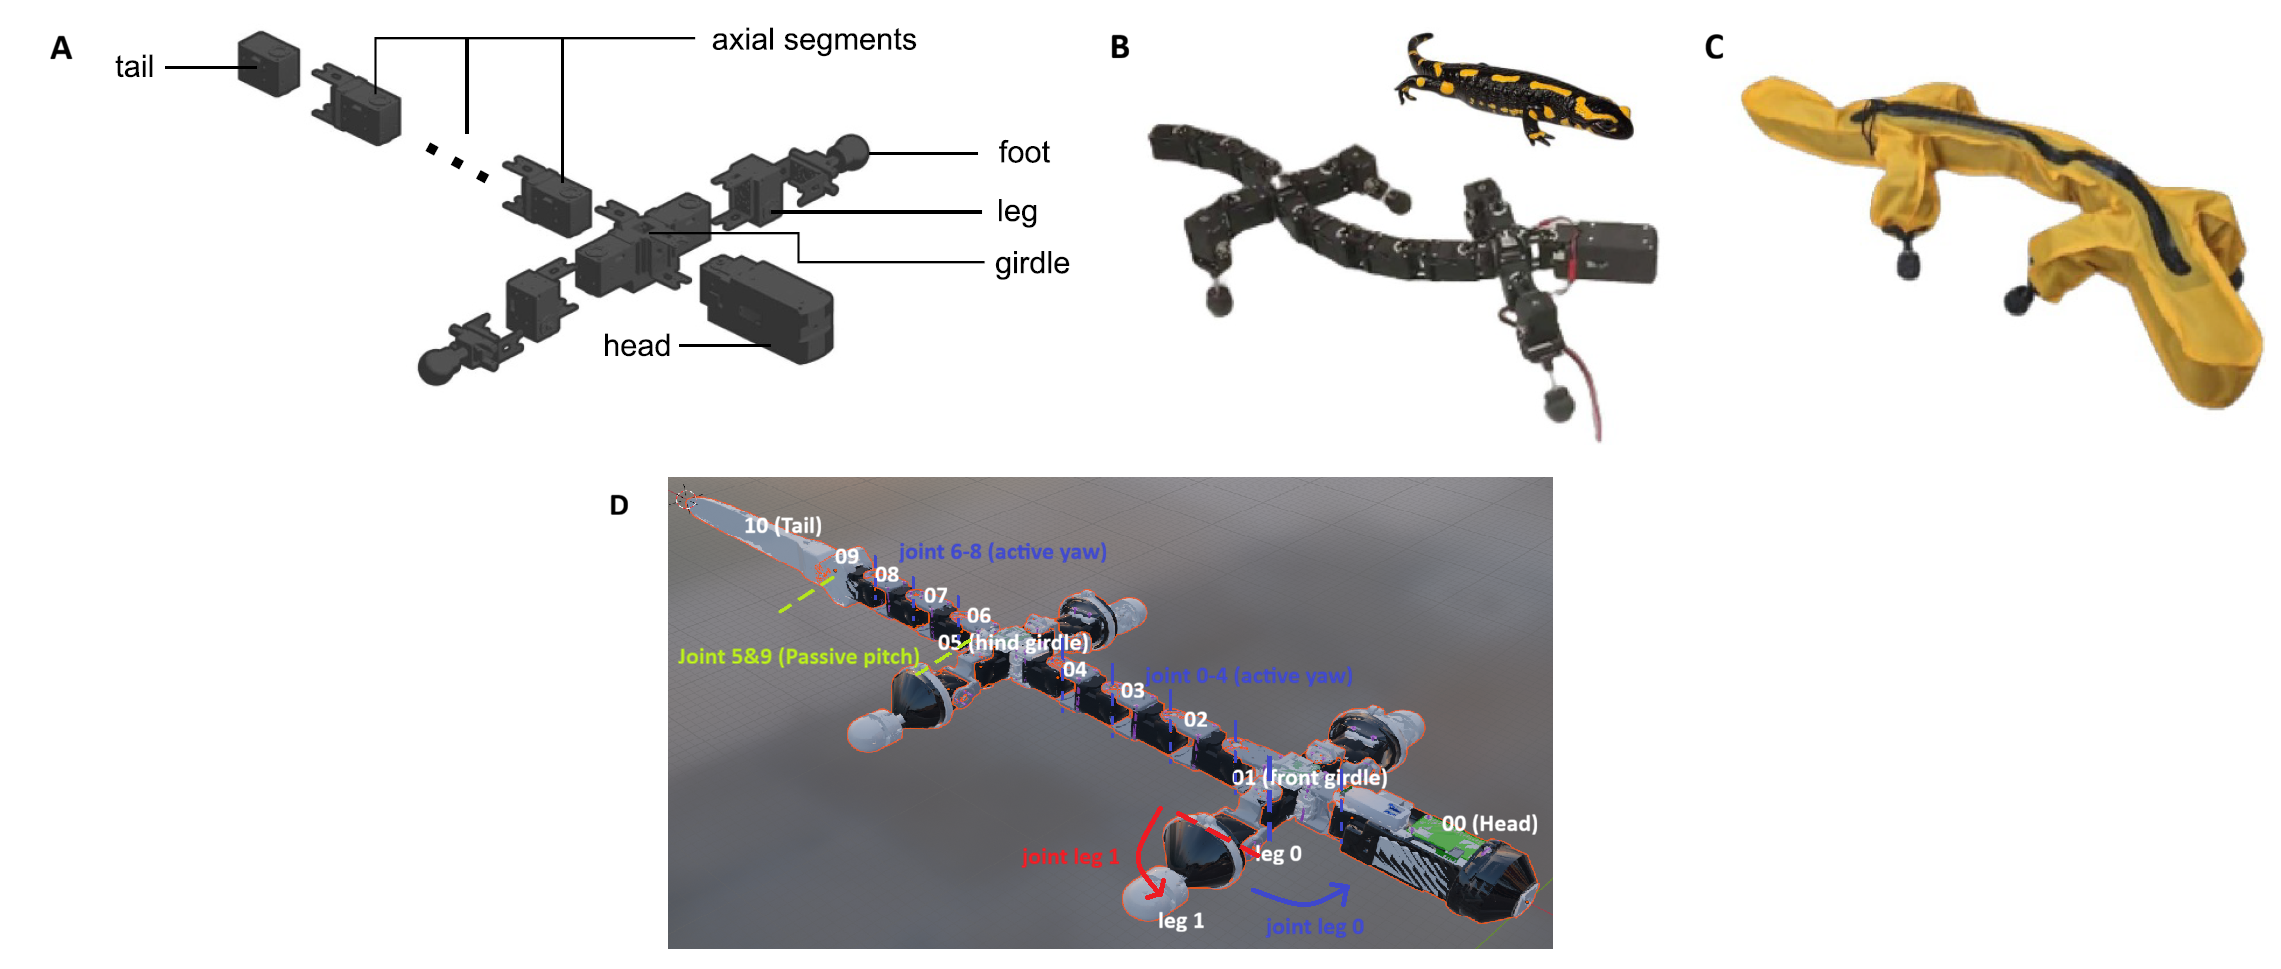
\includegraphics[width=\textwidth]{figures/Polymander robot.png}}
    \caption{Polymander Robot. (A) Reconfigurable modules of the robot. (B) Salamander configuration with two forelimbs and two hindlimbs. (C) Polymander inside its waterproof suit. (D) Links and joints definition of Polymander in the quadruped plan.}
\end{figure}

\begin{figure}[H]
  \centering 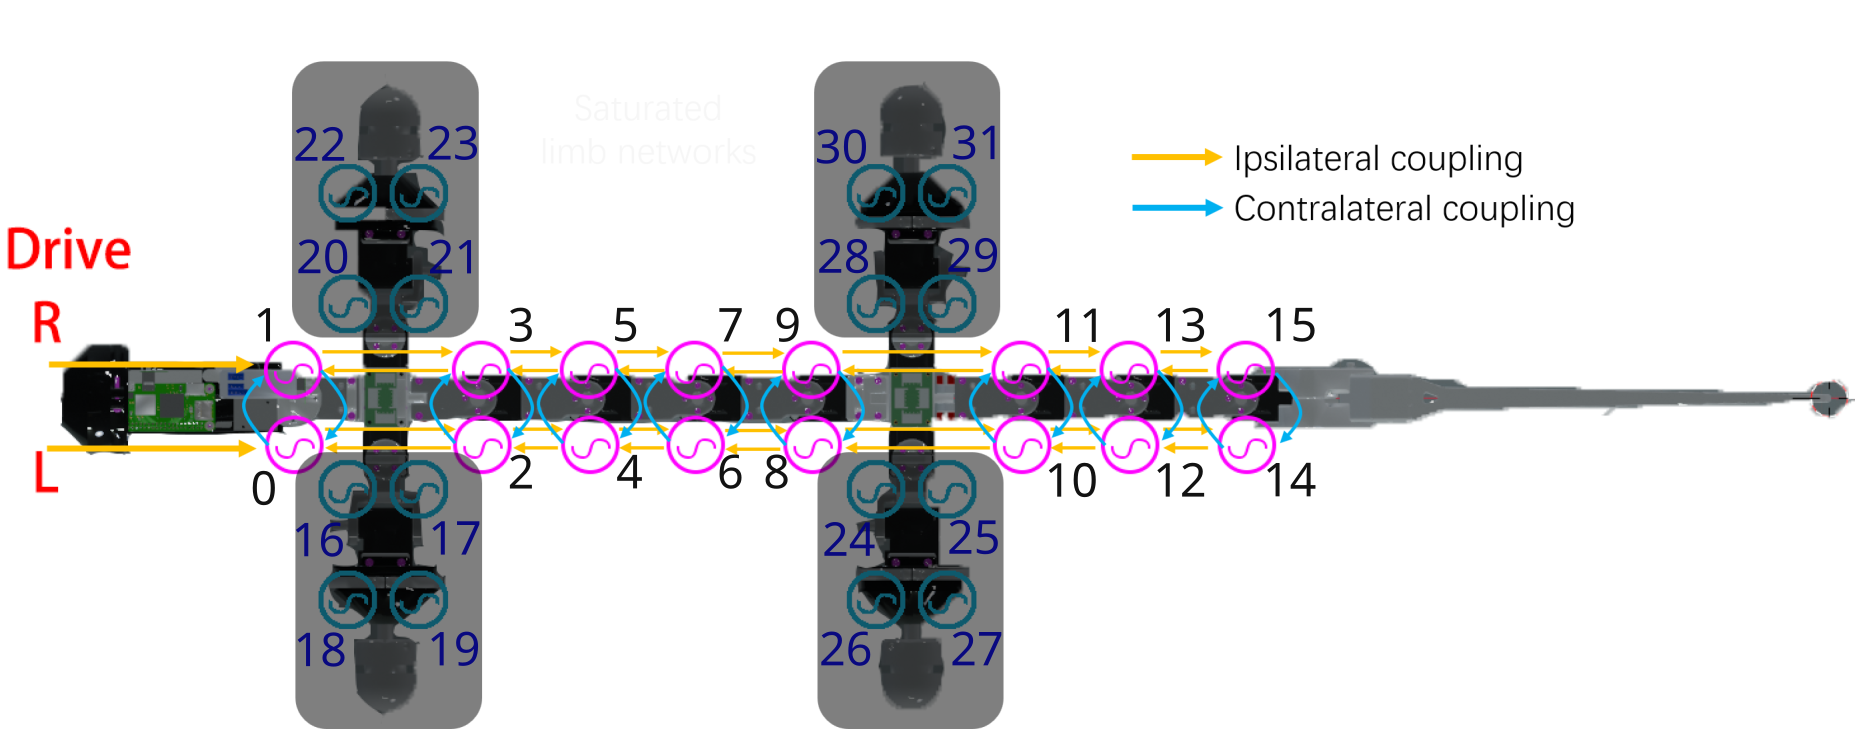
\includegraphics[width=.8\textwidth]{figures/network_indices.png}
  \caption{\label{fig:model_controller} Configuration of the CPG controller in Polymander with oscillator indices. Limb networks will now be considered in Project 2. All joints are driven by pairs of antagonist Ekeberg muscles receiving motor outputs from a pair oscillators. The CPG model receives descending signals from the drive representing the brain MLR region in real animals.}
\end{figure}

\begin{figure}[ht]
  \centering 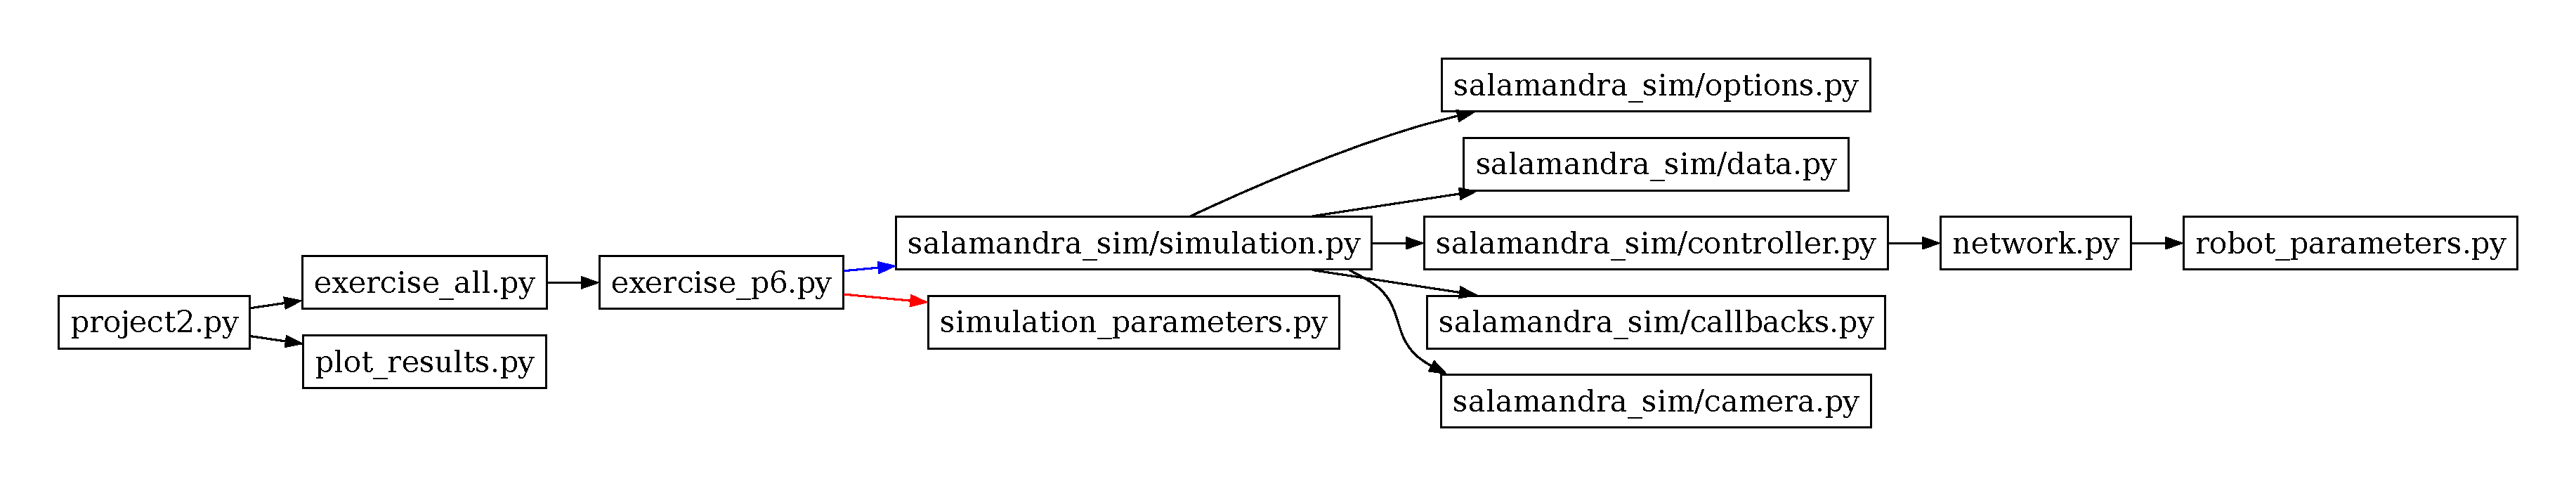
\includegraphics[width=1.0\textwidth]{figures/files}
  \caption{\label{fig:files} Exercise files dependencies. In Part A, you will
    be modifying \fileref{exercise\_p1.py} and \fileref{exercise\_p2.py}, \fileref{network.py},
    \fileref{robot\_parameters.py} and \fileref{simulation\_parameters.py}. Part B will be distributed next week, subject to final validation, and may include additional exercise files.}
\end{figure}

% \newpage

\subsection{Code Structure}

The code is hosted at \texttt{https://gitlab.com/farmsim/courses/cmc-2026-students}. The \texttt{README.md} gives details on the installation.

\subsection*{Code organization}\label{subsec:code}

This project uses the same packages as Project 1. For installation instructions, refer to Project 1 and the \texttt{project\_installation/} directory for installing FARMS and the needed packages.

\begin{itemize}
\item \corr{\textbf{project2.py}} --- A convenient file for running the exercises. Note you can also run the different exercises in parallel by
  activating \texttt{parallel=True}. \textit{You do not need to modify this
    file.}
\item \corr{\textbf{exercise\_all.py}} --- Another convenient file for running all
  or specified exercises depending on arguments provided. \textit{You do not
    need to modify this file.}
\item \corr{\textbf{network.py}} --- This file contains the different classes and
  functions for the CPG network and the Ordinary Differential Equations
  (ODEs). Note that some parameters can be obtained from robot\_parameters.py to help you control
  the values. \textit{You do not need to modify this file.}
\item \corr{\textbf{robot\_parameters.py}} --- This file contains the different
  classes and functions for the parameters of the robot, including the CPG
  network parameters. You can implement the network parameters here. Note that
  some parameters can be obtained from the SimulationParameters class in
  \corr{simulation\_parameters.py} and provided in \corr{exercise\_\#.py} to
  help you control the values (refer to example.py).
\item \corr{\textbf{simulation\_parameters.py}} --- This file contains the
  SimulationParameters class and is provided for convenience to send parameters
  to the setup of the network in \corr{network.py::SalamandraNetwork} via the
  robot parameters in \corr{robot\_parameters.py::RobotParameters}. The
  SimulationParameters is also intended to be used for experiment-specific
  parameters for the exercises. All the values provided in SimulationParameters
  are logged for each simulation, so you can also reload these parameters when
  analyzing the results of an experiment.
\item \corr{\textbf{exercise\_p1.py} and \textbf{exercise\_p2.py}} --- To be used to implement and answer the
  respective exercise questions for Part A. Note that \corr{exercise\_example.py} is
  provided as an example to show how to run a simulation. Note how network
  parameters can be provided here. Part B will be distributed next week, subject to final validation, and may include additional exercise files.
\item \corr{\textbf{exercise\_all.py}} --- A convenient file for running different
  exercises depending on arguments. See \corr{\textbf{project2.py}} for an example
  on how to call it. \textit{You do not need to modify this file.}
\item \textbf{salamandra\_simulation folder} --- Contains all the remaining
  scripts for setting up and running the simulation experiments. \textit{You do
    not need to modify any of these file but should still go through them to get
    a better understanding of the code.}

\end{itemize}

\subsection*{Examples}

You can run a simulation example to get you accustomed
to the MuJoCo graphical interface with \corr{\textbf{exercise\_example.py}}. You
should see the polymander model floating on the water. Try running:
\label{sec:mujoco-example}
\begin{lstlisting}[language=Bash]
  >> python exercise_example.py
\end{lstlisting}

\corr{\textit{IMPORTANT:}} Make sure you have activated and are using your
virtual environment and its python interpreter that that you have created for
this course.

\subsection{Submission}
\textbf{Deadline:} The Project 2 (Parts A and B) needs to be handed in by \corr{\textbf{\underline{Friday, 05.06.2026 at 23:55.}}}

\textbf{Note:} Part B will be distributed next week, subject to final validation, and must be submitted together with Part A.

When submitting, zip your report and your code together as
\nolinkurl{cmc_project2_group_{group_number}.zip}, using your group
number in the filename. Your code should include code files only. The
virtual environment (e.g.\ the \texttt{venv} directory), the
\texttt{farms} folder, and the \texttt{logs} folder should
\textcolor{red}{not} be included. Videos and presented results in the
report should be reproducible by running the main exercise scripts.
Videos should have assignment numbers as prefixes and descriptive
phrases as suffixes that you refer to in your report.
Videos should have descriptive names and be described in the report.

% \newpage

\subsection*{Pro tips}

\begin{itemize}
\item Exercise 1 (Network \& Dynamics) is the most time-consuming and necessary for the remaining exercises. Please manage your time accordingly.
\item Provide a brief explanation of your implementation in each exercise, particularly for Exercise 1.
\item Explain your observations and graphs whenever possible.
\item Try to find metrics for evaluation that can help you explain behaviour in simulations.
\item Focus on biological comparisons, they are required deliverables.
\item Create videos early to demonstrate key behaviors.
\end{itemize}

%%%%%%%%%%%%%%%%%%%%%%%%%%%%%%%%%%%%%%%%%%%%%%%%%%%%%%%%%%%%%%%%%%%%%%%%%%%%%%%%%%%%%%%%%%%%%%%%%%%

\newpage
\section {Assignment}
At this point you can now start to work on implementing your exercises for Part A.
The exercises are organized in a scaffolded progression:

\begin{enumerate}
\item \textbf{Exercise 1 (Network \& Dynamics)}: Implement the full CPG network (axial + limbs) and analyze its dynamics without physics simulation.
\item \textbf{Exercise 2 (Capabilities)}: Connect your CPG to robot physics and demonstrate basic locomotion (walking).
\end{enumerate}

You will first implement the oscillator network model in \corr{robot\_parameters.py} (you can use \corr{simulation\_parameters.py} to handle variables that change between experiments) and run it using \corr{exercise\_p1.py} with \corr{run\_network} function and analyze it. Exercise 1 describes the questions needed to implement the oscillator models. After completing exercise 1 you should have an oscillator network including both the axial and limb CPG.\@ Using the network implemented in Exercise 1, you will explore its capability to perform walking and transitions in MuJoCo (Exercise 2).

\textbf{Note:} Part B of Project 2, containing additional exercises, will be distributed next week, subject to final validation. Part A and Part B will need to be submitted together.

Note: in addition to the explanations for each question below there are more explanations in the code.
Check the commented code in each relevant file!

% EXERCISE 1 %%%%%%%%%%%%%%%%%%%%%%%%%%%%%%%%%%%%%%%%%%%%%%%%%%%%%%%%%%%%%%%%%%%%%%%%%%%%%%%%%%%%%%%%%%%%%%%%%%%

\subsection{Exercise 1: Network \& Dynamics}\label{sec:network-implementation}

In this exercise, you will implement the full CPG network (axial + limbs) and analyze its dynamics without physics simulation.

Polymander has 8 joints along its spine and 2 joints for each limb. As in Project 1, we use a double chain of oscillators for axial actuation, where each spine joint is governed by two oscillators. For the limbs, we also use pairs of oscillators (two per joint) since they are muscle-controlled with antagonist muscles described by the Ekeberg model. The same oscillator phase and amplitude equations (Eqs. \ref{eq:dphase} and \ref{eq:dr}) govern both axial and limb joints, but note that the oscillator parameters differ between axial and limb oscillators (see supplementary material of \cite{ijspeert2007swimming}).

The oscillator phase equation is defined in Eq.\ref{eq:dphase}, with $ \phi_i $ the oscillator phase, $f_i$ the oscillator intrinsic frequency, $ w_{ij} $ the coupling weights, $ \psi_{ij} $ the nominal phase lag (phase bias), and $ r_i $ the oscillator amplitude.

\begin{equation}
  \label{eq:dphase}
  \dot{\phi}_i = 2 \pi f_i + \sum_j r_j w_{ij} sin(\phi_j - \phi_i - \psi_{ij})
\end{equation}

The oscillator amplitude equation is defined in Eq.\ref{eq:dr}, where $r_i$ is the oscillator amplitude, $R_i$ is the nominal amplitude, and $a_i$ is the convergence rate.

\begin{equation}
  \label{eq:dr}
  \dot{r}_i = a_i (R_i - r_i)
\end{equation}

The muscle output of a axial and limb oscillator are both defined as a function of oscillator phase and amplitude in Eq.~\ref{eq:output_oscillator}.

\begin{equation}
  \label{eq:output_oscillator}
  M_i = r_i(1 + cos(\phi_i))
\end{equation}

\begin{enumerate}
\item \textbf{Part A (Network Implementation):} Implement the full CPG network (axial + limbs). Adapt the double chain oscillator model from Project 1 for the axial CPG ($i=[0, \ldots, 15]$), and extend it to include limb circuits ($i=[16, \ldots, 32]$). Note that unlike Ijspeert 2007 (which used one oscillator per limb), our robot has 2 joints per limb requiring 4 oscillators (2 pairs of antagonists). The connectivity for these limb oscillators is an open question: you must design and justify your proposed architecture to replicate the gaits from Ijspeert 2007 with our higher-DoF robot. Start by considering: (1) the relationship between antagonist muscles for each joint, (2) the phase shift between the two limb joints (girdle and elbow/knee) for circular motion, and (3) the coordination between limbs and with axial oscillators. Test your implementation using \fileref{exercise\_p1.py}. For network parameters, check the supplementary material \cite{ijspeert2007swimming}. Note that parameters will need to be slightly adapted for our higher-DoF robot, and you should explain your choices. Refer to \corr{salamandra\_simulation/data.py::SalamandraState} and \corr{robot\_parameters.py} for the state and network parameter dimensions. For the muscle output, implement the axial and limb oscillator output according to Eq.~\ref{eq:output_oscillator}.

\item \textbf{Part B (Network Dynamics Validation):} Implement a drive that linearly increases from 0 to saturation (e.g., 0 to 6 over 20 seconds). Your plots should reproduce patterns similar to Figures \ref{fig:science_oscillator_patterns} and \ref{fig:science_oscillator_properties}.
  \textbf{Hint:} The state for the network ODE is of size 64 where the first 32 elements correspond to the oscillator phases $\phi_i$ and the last 32 elements correspond to the amplitude $r_i$. The initial state is set in the init of \corr{network.py::SalamanderNetwork}.
\end{enumerate}

\begin{figure}[H]
  \centering
  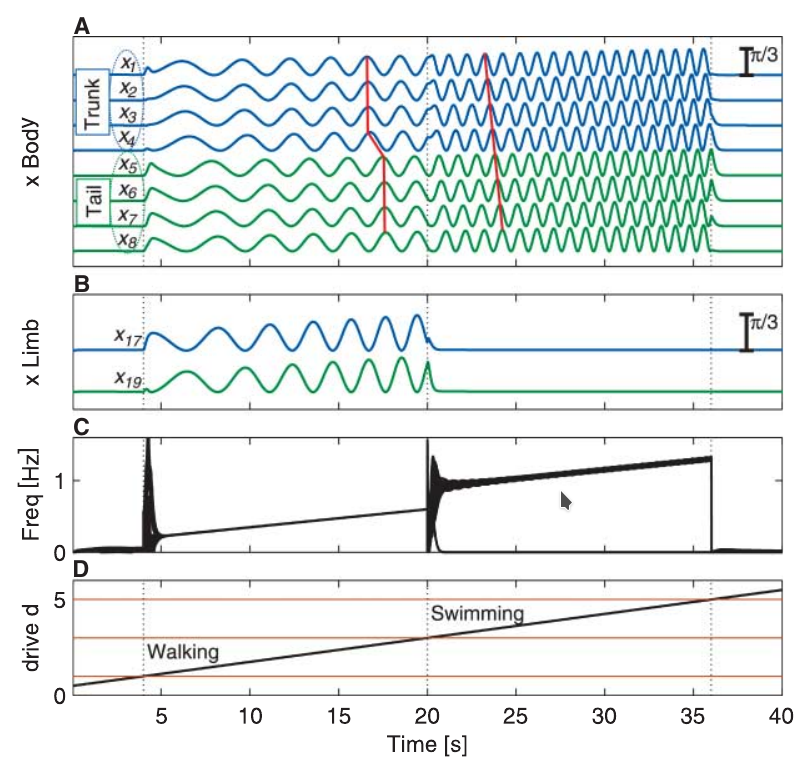
\includegraphics[width=0.7\textwidth]{figures/science_oscillator_patterns}
  \caption{Oscillator patterns from~\cite{ijspeert2007swimming}, see~\cite{ijspeert2007swimming} for details}\label{fig:science_oscillator_patterns}
\end{figure}

\begin{figure}[H]
  \centering
  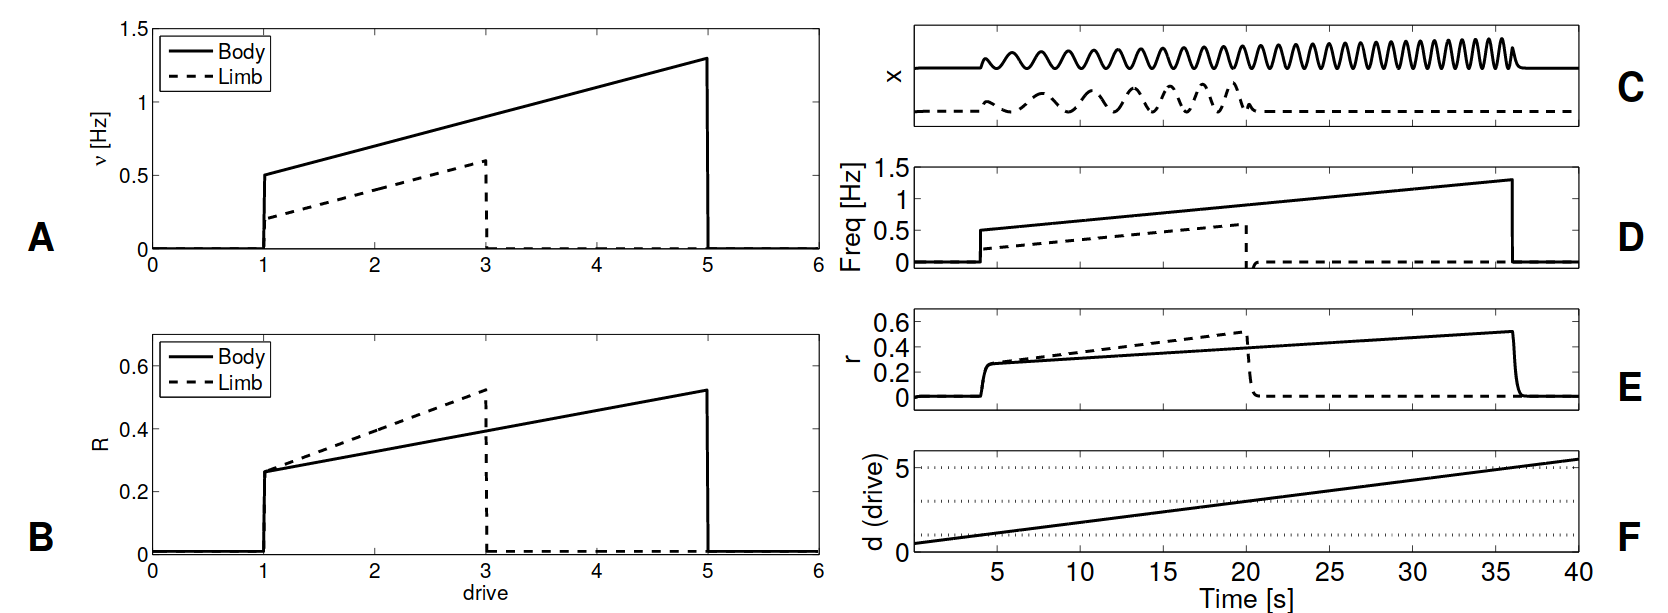
\includegraphics[width=1.0\textwidth]{figures/science_oscillator_properties}
  \caption{Oscillator properties from~\cite{ijspeert2007swimming} supplementary
    material, see~\cite{ijspeert2007swimming} for details}\label{fig:science_oscillator_properties}
\end{figure}

%% -----------------------------SOLUTION EXERCISE 1 ------------------------------

% %%%%%%%%%%%%%%%%%%%%%%%%%%%%%%%%%%%%%%%%%%%%%%%%%%%%%%%%%%%%%%%%%%%%%%%%%%%%%%%%%%%%%%%%%%%%%%%%%%%%%%%%%%%%%%
% EXERCISE 2 %%%%%%%%%%%%%%%%%%%%%%%%%%%%%%%%%%%%%%%%%%%%%%%%%%%%%%%%%%%%%%%%%%%%%%%%%%%%%%%%%%%%%%%%%%%%%%%%%%%
\newpage
\subsection{Exercise 2: Capabilities}\label{sec:capabilities}

In this exercise, you will connect your CPG network to robot physics and demonstrate basic locomotion.

\begin{enumerate}
\item \textbf{Part A (Physics Integration):} Run your controller in the physics simulation. Validate that your CPG network from Exercise 1 (now including limb circuits) works with the Polymander robot model for walking.
  \textbf{Deliverable:} Video (10--15 seconds) showing the robot walking with default parameters.

\item \textbf{Part B (Drive Ramp Experiment):} Run a simulation with drive linearly increased from minimum to maximum values over about 40 seconds. Perform this experiment on flat ground and in water.
  \textbf{Deliverable:} Videos (about 40 seconds each) of robot behavior during drive ramp (side view) for both environments. You may reuse plots from Exercise 1 for comparative discussion. Describe the sequence of gaits observed, name them, discuss their usefulness depending on the environment, and explain which gaits observed in salamanders are not exhibited by the robot and why. Hypothesize what might be missing in the model to elicit these other gaits. Discuss how the brain could recruit these gaits depending on its needs.
\end{enumerate}

% %%%%%%%%%%%%%%%%%%%%%%%%%%%%%%%%%%%%%%%%%%%%%%%%%%%%%%%%%%%%%%%%%%%%%%%%%%%%%%%%%%%%%%%%%%%%%%%%%%%%%%%%%%%%%%
% EXERCISE 2 %%%%%%%%%%%%%%%%%%%%%%%%%%%%%%%%%%%%%%%%%%%%%%%%%%%%%%%%%%%%%%%%%%%%%%%%%%%%%%%%%%%%%%%%%%%%%%%%%%%

%%%%%%%%%%%%%%%%%%%%%%%%%%%%%%%%%%%%%%%%%%%%%%%%%%%%%%%%%%%%%%%%%%%%%%%%%%%%%%%%%%%%%%%%%%%%%%%%%%%%

%%%%%%%%%%%%%%%%%%%%%%%%%%%%%%%%%%%%%%%%%%%%%%%%%%%%%%%%%%%%%%%%%%%%%%%%%%%%%%%%%%%%%%%%%%%%%%%%%%%%

% \newpage

% NOTE: Use this for .bib file instead of listing the \bibitems in the bibliography
% \bibliographystyle{ieetr}
% \bibliography{project1}\label{sec:references}

\begin{thebibliography}{9}

  % Volume, Number, Page, Month, Year
  \bibitem{Crespi2013}
  A. Crespi and K. Karakasiliotis and A. Guignard and A. J. Ijspeert,
  \emph{Salamandra Robotica II:\ An Amphibious Robot to Study Salamander-Like Swimming and Walking Gaits},
  IEEE Transactions on Robotics, Vol. 29, Num. 2, pp.308--320, April 2013,

  \bibitem{Karakasiliotis2013}
  Karakasiliotis, Konstantinos and Schilling, Nadja and Cabelguen, Jean-Marie and Ijspeert, Auke Jan,
  \emph{Where are we in understanding salamander locomotion: biological and robotic perspectives on kinematics},
  Biological Cybernetics, Vol. 107, Num. 5, pp. 529--544, October 2013,

  \bibitem{ijspeert2007swimming}
  Ijspeert, Auke Jan and Crespi, Alessandro and Ryczko, Dimitri and Cabelguen, Jean-Marie,
  \emph{From swimming to walking with a salamander robot driven by a spinal cord model},
  Science, Vol. 315, Num. 5817, pp. 1416--1420, 2007

  \bibitem{thandiackal2021emergence}
  Thandiackal, Robin and Melo, Kamilo and Paez, Laura and Herault, Johann and Kano, Takeshi and Akiyama, Kyoichi and Boyer, Fr{\'e}d{\'e}ric and Ryczko, Dimitri and Ishiguro, Akio and Ijspeert, Auke J,
  \emph{Emergence of robust self-organized undulatory swimming based on local hydrodynamic force sensing},
  Science Robotics, Vol. 6, Num. 56, pp.\ eabf6354, 2021,

  \bibitem{owaki2013simple}
  Owaki, Dai and Kano, Takeshi and Nagasawa, Ko and Tero, Atsushi and Ishiguro, Akio,
  \emph{Simple robot suggests physical interlimb communication is essential for quadruped walking},
  Journal of The Royal Society Interface, Vol. 10, Num. 78, pp. 20120669, 2013,

\end{thebibliography}

% \newpage

% \section*{APPENDIX}
% \label{sec:appendix}

\end{document}

%%% Local Variables:
%%% mode: latex
%%% TeX-master: t
%%% End:
